\section{Current contributions}

\subsection{Proof of Concept}


\begin{itemize}
    \item T.~Vintr, S.~Molina, J.~Fentanes, G.~Cielniak, T.~Duckett, and T.~Krajn{\'i}k, ``Spatio-temporal models for motion planning in human populated environments,'' in \emph{Student Conference on Planning in Artificial Intelligence and Robotics}, 2017.
\end{itemize}

In [výše] we propose a method that allows to capture the natural daily and weekly periodicities of human presence (imposed by daily habits of going to work, cleaning, etc) in different areas of space.
Our approach proposes to extend continuous spatial representations by adding several dimensions representing different periodicities in time. 
In particular, we transform every time periodicity into two new dimensions that form a circle in its $2D$ subspace and use them to extend the representations that model $2D$ or $3D$ space. 
The model is then built using traditional clustering over the resulting spatio-temporal hyperspace, which efficiently represents both the structure of the space (given by environment) and time (given by the human habits).
Unlike \cite{krajnik2017fremen} that can identify and represent multiple periodicities, we decided to model only the daily one for the sake of simplicity.

To extend a continuous spatial representation we have to create new time dimensions.
We transform the time values $t$ into two new dimensions

\begin{equation}\label{trans_cos}
\begin{array}{ccc}
    t_c& = &\cos{2\pi \omega t},\\
    t_s& = &\sin{2\pi \omega t},
\end{array}
\end{equation}

\noindent where $\omega$ corresponds to the chosen periodicity.
The measured vectors $\mathbf{\chi} = (x, y, t)$ are transformed into vectors $\mathbf{x} = (x, y, t_c, t_s),$ which generate a new $4D$ hyperspace. 
The set of vectors $\mathbf{\tau} = (t_c, t_s)$ lies on a  circle  in its $2D$ subspace.


For the purposes of creating the $4D$ continuous model we have chosen from the list of well-known clustering methods~\cite{kruse2007fundamentals} the Gustafson--Kessel Algorithm~\cite{gustafson1979fuzzy}. 


To evaluate the presented approach, we used data about people presence collected at one of the corridors of the School of Computer Science at the University of Lincoln.
Data collection was performed by a mobile robot equipped with a Velodyne 3d laser range-finder.
The robot was placed at a T-shaped junction so that its laser range-finder was able to scan the three connecting corridors simultaneously.
To detect and localize people in the 3d point clouds provided by the scanner, we used an efficient and reliable person detection method~\cite{yan2017online}.
Since we needed to recharge the robot occasionally, we did not collect data about people presence on a 24/7 basis, but we recharged the robot batteries during nights, when the building is vacant and there are no people in the corridors.
Thus, our dataset spanned from early mornings to late evening over several weekdays.
Each day contains approximately $28000$ entries, which correspond to hundreds of people walking or standing in the monitored corridors. 

As a natural period of time to prove this concept we have chosen one day. Parameters for clustering algorithm were chosen as: fuzzifier $m = 2,$ number of clusters $k = 30.$ 

\begin{figure}[!t]
   \begin{center}
      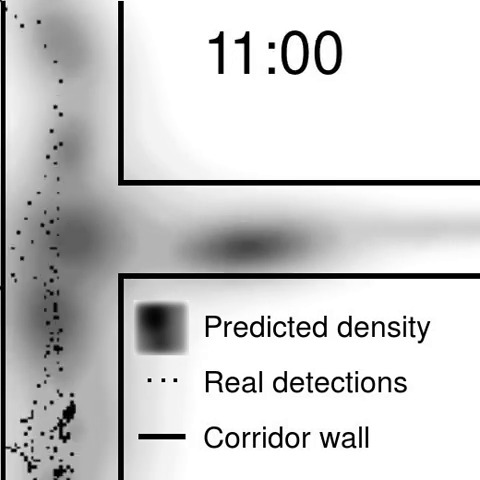
\includegraphics[width=0.3\columnwidth]{fig/corridor_0}
    \hfill
      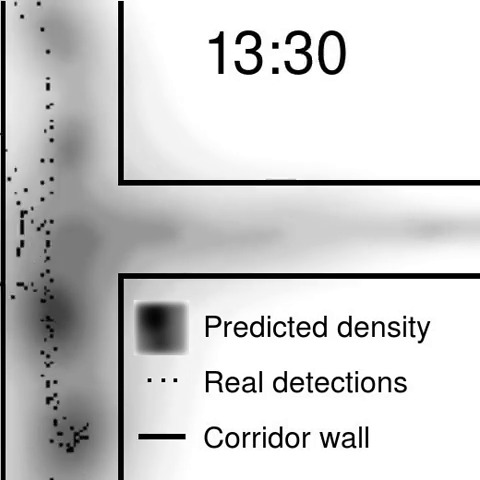
\includegraphics[width=0.3\columnwidth]{fig/corridor_1}\\\vspace{5mm}
      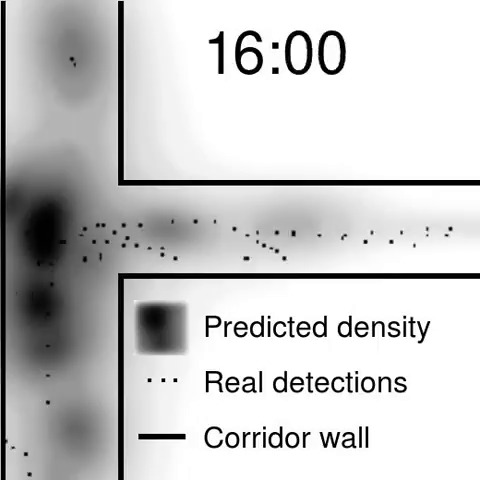
\includegraphics[width=0.3\columnwidth]{fig/corridor_2}
    \hfill
      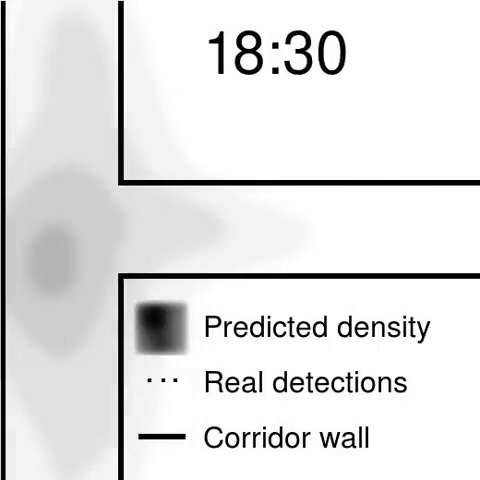
\includegraphics[width=0.3\columnwidth]{fig/corridor_3}
      \caption{Screen grab from the video available at~\url{https://youtu.be/4SW4j7DDxYE}.\label{screen}}
   \end{center}
\end{figure}


To evaluate the model qualitatively we have chosen visualization in the form of a video, see Figure~\ref{screen}. The video visualises measured positions of people, and the probabilistic distribution of their presence generated by our model. 
Every frame of the video projects one time frame. The time step is chosen to be $5$ minutes, and the whole video comprises two days of measurements. Time values are placed in the form of text on the bottom left part of the video screen. It is obvious that the model outputs correlate with the human behavior in the selected space.



\subsection{Warped Hypertime}

\begin{itemize}
    \item Spatiotemporal models of human activity for robotic patrolling
\end{itemize}

The aim of the method [výše] is to create a model of human presence in the patrolling robot operational area.
Such a model has to predict the regular behaviour and incorporate the detection of anomalous events. 
Anomalous events, outliers in data, and novelties in streams of data are defined only vaguely as measurements, that are somehow strange -- unexpected, inconsistent, suspicious, or rare -- compared to the previous experience of a human observer \cite{grubbs1969procedures}, \cite{barnett1974outliers} and there are many approaches to solve different scenarios in different scientific fields \cite{ilango2012five}. 
In our case, we use the outlier detection based on the model \cite{rousseeuw2005robust}. 
Our model is a function that estimates the Bernoulli distribution \cite{evans20004} of occurrences over the time line -- similarly to FreMEn model \cite{krajnik2014spectral,krajnik2017fremen,coppola2016learning}.

For the time dependent events prediction we usually use methods for time series forecasting.
The time series forecasting understands time-dependent events as a combination of three components that can be analysed separately - a trend, seasonal and cyclic patterns \cite{hyndman2018forecasting}.
The trend describes long-term increase or decrease in data, seasonal patterns describe periodical changes in data and cyclic patterns are fluctuations in data with unknown periodicity.
In the proposed method we assume that it is possible to neglect the trend and cyclic patterns due to the nature of the studied problem, where the environmental changes are induced directly by human routines and habits.
Therefore, our model is derived from periodical patterns, that explain the majority of events in human populated environment. 
Using the time series forecasting with neglected trend to analyse the time dependent human behaviour patterns was firstly introduced in \cite{krajnik2017fremen} and it demonstrated its efficiency in different robotic applications and scenarios \cite{fentanes2015now,krajnik2015s,santos2016lifelong}.

Contrary to usual approach of modelling multiple seasonalities, where individual patterns are analysed separately \cite{gould2008forecasting}, we create a special vector space, that reflects every selected seasonality, project the time series into it, and then analyse the periodical features of human behaviour in that space, see Fig.~\ref{fig:hypertime}.
Similarly to \cite{vintr2017spatiotemporal}, for every seasonal pattern we create extra two dimensions and project the time series into a circle on that plane in the way that every measurement from the same position relative to the periodicity is on the same position on the circle.
The proposed projection then reflects not only the seasonality derived from the structure of the vector space, but also the continuity derived from a circularity of the projection.

Our method supposes that there are some patterns -- functions derived from the human behaviour -- over the time line.
To create models of different features in data, we need to estimate parameters of their distributions.
But the time line, understood as domain of some time dependent function, is not suitable to estimate the distribution
of features that occur rarely, because we cannot repeatedly observe the same situation.
As we assume the periodical nature of these features, we can transform the time line into the different, constrained vector space.
The idea behind this transformation is based on the following hypothesis: the human  behaviour is very similar during every morning as opposed to the difference in behaviour during morning and afternoon of one randomly chosen day.
Similarly, human behaviour five minutes before midnight and five minutes after midnight could be probably very similar, although in fact we compare behaviour in two different days.
Contrary to that, human behaviour during Sunday afternoon is probably different from behaviour on Monday afternoon, etc.
Therefore, our method transforms time line into the set of circles based on chosen periodicities detected in data, see Fig. 1.
For example, when it chooses periodicity of one day, every measurement from the dataset is projected into this circle in a way that measurements from the same time in different days are at the same position.
Than we can study periodical features of human behaviour with chosen periodicity and estimate distribution parameters, as illustrated in Fig.~\ref{fig:hypertime}.
It is possible to extend this vector space with new dimensions and project data into the corresponding circles.
We call this vector space with such projection of data the \textit{warped hypertime}.
When the model of mixture of distributions over warped hypertime is created, we can define regular and anomalous human behaviour in the robot's operational area.

\begin{figure}[h]
\begin{center}
    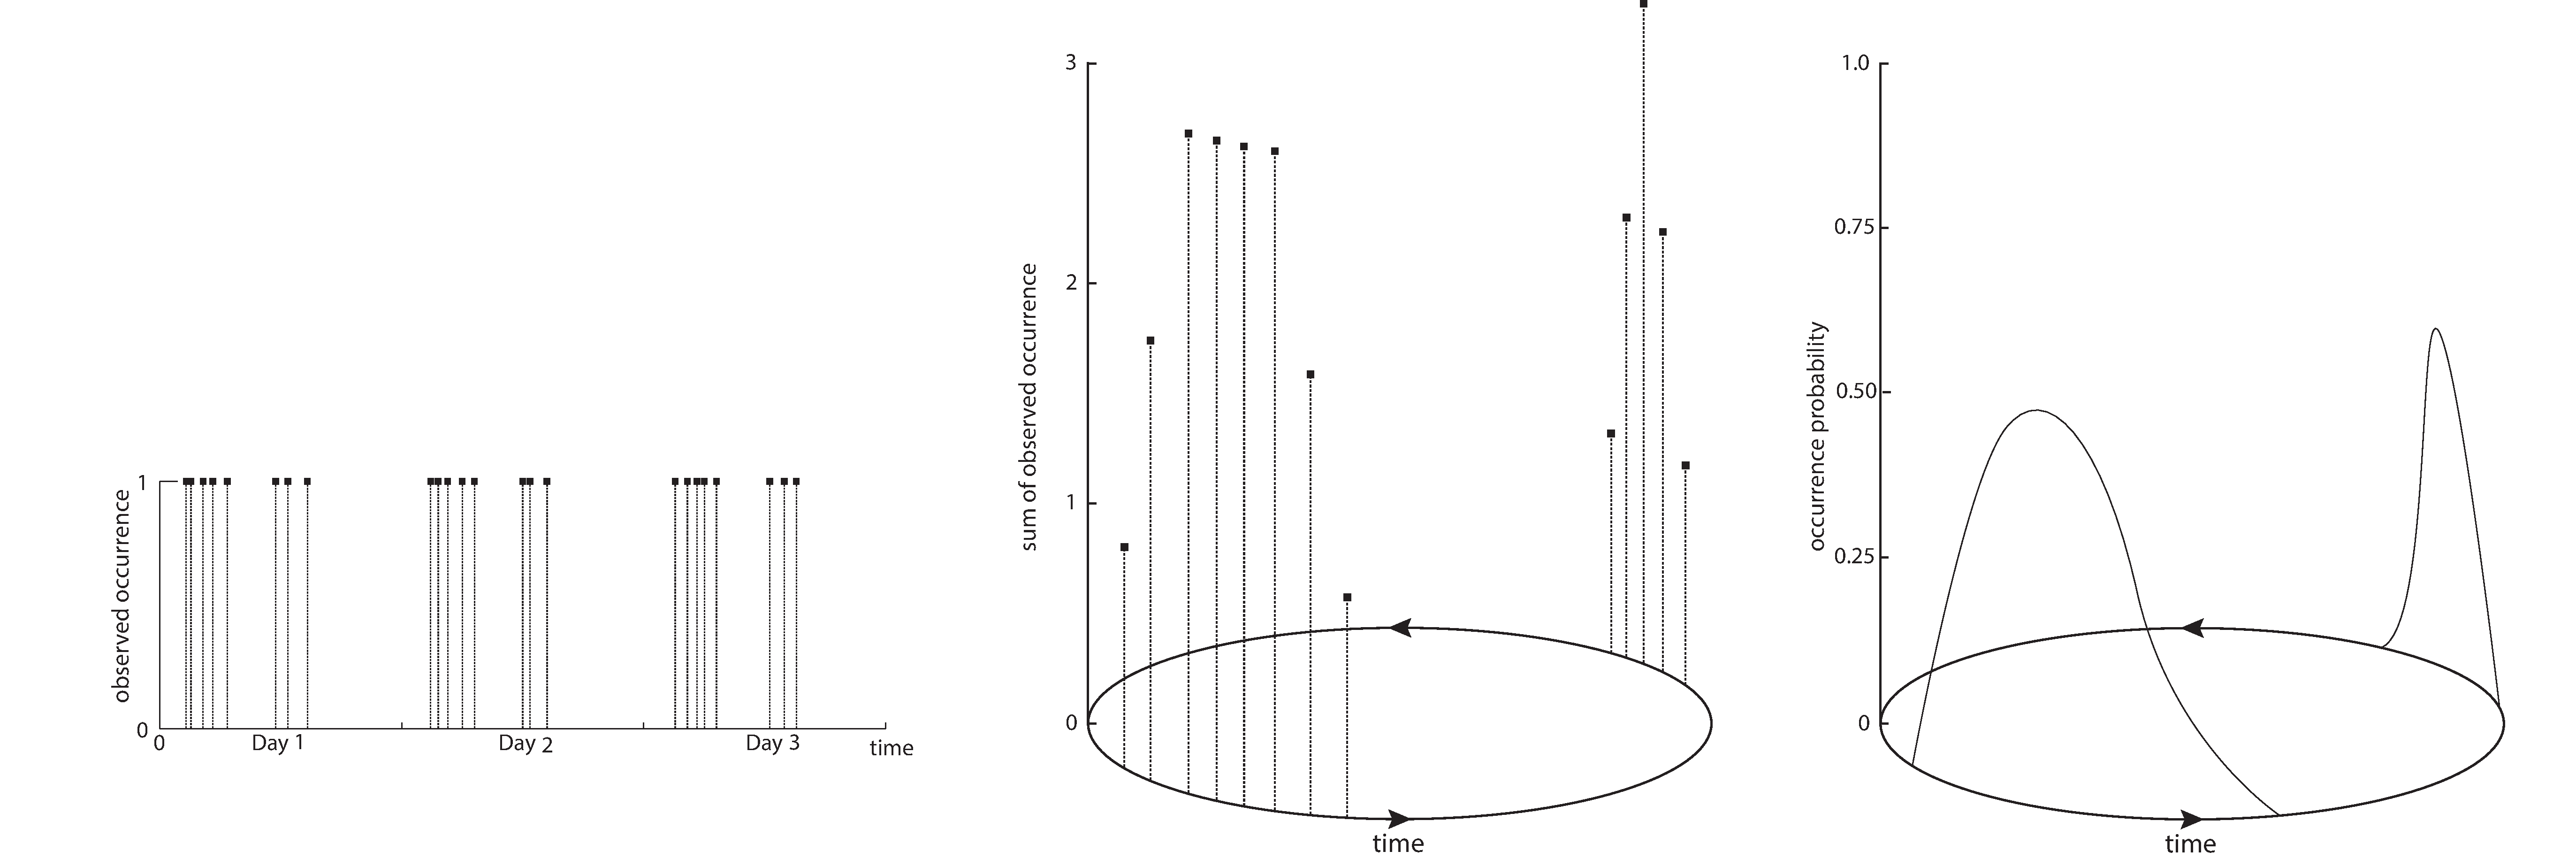
\includegraphics[width=1.0\columnwidth]{fig/hypertime_graph}
    \caption{Example of the warped hypertime projection. Positive detections during three days are projected into a warped hypertime with a one day period. The parameters of the distribution of a random time dependent phenomenon that exhibit a periodic behaviour can be easily estimated.\label{fig:hypertime}}

\end{center}
\end{figure}


The detection of the most influencing periodicities in the data can be done using the Spectral analysis \cite{brockwell2016introduction}, parameters of the mixture of distributions can be gathered using the Expectation-Maximisation model for Gaussian mixtures \cite{xu1996convergence} and parameters of distribution of residuals between model and measured data for anomaly detection can be obtained using the robust descriptive statistic \cite{maronna2006robust}. 

We evaluated our method on a real world dataset from Lincoln university. 
It consists of twenty weeks of detection of one person in his office.
We divided this dataset into the training dataset that consists of first three weeks
% (Fig. \ref{graph:3weeks})
 and the test dataset that consists of the eighteenth week.% (Fig. \ref{graph:outliers}).
We compare our method, warped hypertime technique \textit{WHyTe}, with four different methods.
First of them is \textit{Prophet}, the open source time series analysis tool created by Facebook \cite{taylor2018forecasting}, second is \textit{FreMEn} as defined in \cite{krajnik2017fremen} using five most influencing periodicities, and the last two are histograms \textit{Hist24} and \textit{Hist168}.
Hist24 calculates the mean of occurrences for every hour in a day and Hist168 calculates one hour means over the whole week.

WHyTe needed shorter time to learn features of the studied subject behaviour than the other methods.
The ability of WHyTe to detect the anomalous behaviour on our dataset is significantly better than the ability of FreMEn.
Compared to the other methods, WHyTe exhibits robustness to the choice of significance level.
Moreover, WHyTe is better compared to the popular technique in robotics, the histograms, even if these histograms use correctly predefined periodicities. 
Based on our experiments, the assumption that the trend should be neglected for the human behaviour analysis over several weeks was correct.

\subsubsection{Creation of Warped Hypertime in Detail}


Let us have time series $R\left(t_{i}\right)$, $i = 1 \ldots n$, where $R\left(t_{i}\right) = 1$ when the sensor detects an occurrence of the studied phenomenon and $R\left(t_{i}\right) = 0$ otherwise.
Than we use the spectral analysis to find periodicities in the data, specifically we will use the method derived from the Frequency Map Enhancement \cite{krajnik2017fremen}. 
This method is suitable to analyse time series with binary data and it is robust to missing values.
For every considered period $T_{\tau}$, $\tau = 1 \ldots \Upsilon$, corresponding to the frequency ${f}_{\tau} = 1 / T_{\tau}$ we calculate a component of the frequency spectrum

\begin{equation}\label{eq:components}
\gamma_{\tau} = \frac{1}{n} \sum_{i = 1}^{n} (R\left(t_{i}\right)-\mu)e^{(-1j)t_{i}{f}_{\tau}2\pi},
\end{equation}

\noindent where $\mu = \frac{1}{n} \sum_{i = 1}^{n} R\left(t_{i}\right)$, sort them in descending order and return corresponding periods ordered accordingly.


For every chosen period $T_{\tau}$ we can create two $2d$ warped hypertimes -- projections of $R\left(t_{i}\right)$ and $1 - R\left(t_{i}\right)$ into $\left\{t|h(t, T_{\tau})\right\}$ (Fig.~\ref{fig:hypertime}), where the function $h$ is defined as follows:

\begin{equation}\label{eq:hyperime}
    h(t, T_{\tau}) = \left(\cos{\left(\frac{2\pi t}{T_{\tau}}\right)}, \sin{\left(\frac{2\pi t}{T_{\tau}}\right)}\right).
\end{equation}


\noindent The time series $R\left(t_{i}\right)$ reflect detected occurrences of a studied phenomenon and time series $1 - R\left(t_{i}\right)$ reflect complement phenomenon, 'non-occurrences'.
The warped hypertimes with the projection of the same time series can be combined into a warped hypertime of  higher dimension 
\begin{equation}\label{eq:multihyper}
R\left(t_{i}\right) \rightarrow \left\{t|\left(h(t, T_{\tau_1}), h(t, T_{\tau_2}), \ldots\right)\right\}.
\end{equation} 

To identify parameters of the studied phenomenon, we create warped hypertimes and apply the Expectation Maximisation algorithm for estimating Gaussian Mixture Models (EM GMM).
As the periods are ordered by their influence to $R(t_i)$ %(subsection \ref{sec:fremen})
, we can build models in an iterative manner and choose the best one based on the chosen criterion.

Let us denote a warped hypertime $H$, which is build using first $p$ of most influencing periods and with projection of time series $R(t_i)$ as $H(R, p)$ and a model over this space with $c$ clusters as $M(R, p, c)$, then we can describe an iterative process to find the best model as two nested loops, the inner one with growing parameter $p$ (number of periods) and the outer one with growing parameter $c$ (number of clusters). 
The obtained models are compared using the Root-mean-square deviation (RMSD) \cite{hyndman2006another} between the projection of a model to a time line $\hat{R}_{c, p}\left(t_{i}\right)$ and time series $R\left(t_{i}\right)$:

\begin{equation}\label{eq:rmsd}
E_{c, p} = \sqrt{\frac{1}{n}\sum_{i=1}^{n}{\left(\hat{R}_{c, p}\left(t_{i}\right) - R\left(t_{i}\right)\right)^{2}}},
\end{equation}

\noindent where 

\begin{equation}\label{eq:model}
\hat{R}_{c, p}\left(t_{i}\right) = \hat{R}_{c, p}^{*}\left(t_{i}\right) \frac{\sum_{i=1}^{n}{R_{c, p}\left(t_{i}\right)}}{\sum_{i=1}^{n}{\hat{R}_{c, p}^{*}\left(t_{i}\right)}},
\end{equation}

\noindent where

\begin{equation}\label{eq:ratio}
\hat{R}_{c, p}^{*}\left(t_{i}\right) = \frac{\hat{R}_{c, p}^{1}\left(t_{i}\right)}{\hat{R}_{c, p}^{1}\left(t_{i}\right) + \hat{R}_{c, p}^{0}\left(t_{i}\right)}
\end{equation}

\noindent where $\hat{R}_{c, p}^{1}\left(t_{i}\right)$ is a modelled value of occurrence  $M\left(R, p, c\right)$ at time $t_i$ and $\hat{R}_{c, p}^{0}\left(t_{i}\right)$ is a modelled value of non-occurrence  $M\left(1 - R, p, c\right)$ at the same time.
$\hat{R}_{c, p}^{*}\left(t_{i}\right)$ is the estimation of relative frequency of occurrences in time $t_i$, and after application of normalisation (\ref{eq:model}) we can think of $\hat{R}_{c, p}\left(t\right)$ as about the function that estimates probability value of the Bernoulli distribution \cite{evans20004} of a studied phenomenon in time.
The model with the lowest value of $E_{c, p}$ is chosen. 



\subsection{Warped Hypertime Space}

\begin{itemize}
    \item Spatio-temporal representation for long-term anticipation of human presence in service robotics
\end{itemize}

The aim of the proposed method [výše] is to create a spatio-temporal model capable of predicting future human presence across the operational environment of the robot.
As the model is created from data gathered by a real mobile robot over long-time periods, it has to deal with uncertainty of the measurements, occlusions, missing data etc. 
The input data of the model are positions of people provided by a state-of-the-art people detection method based on vision or active sensors, such as~\cite{yan2017online}.
 
Let us assume that every time a robot performs a measurement of the position of a detected person, it obtains a tuple ($\mathbf{x}_i$, $t_i$), where $\mathbf{x}_i$ describes the position and $t_i$ corresponds to the time when the measurement was taken.
Thus, our method aims to find a function $\rho(\mathbf{x},t)$, which characterizes the frequency of occurrence of the vector $\mathbf{x}$ over time.
Contrary to the usual approach to analysis of time series that iteratively decomposes particular patterns, our approach is to create specific projection of tuples ($\mathbf{x}_i$, $t_i$) into a new vector space, and then create a model of frequency of occurrence in this space.  
(As it was said, we assume that there is no long-term trend and neglect cyclic patterns due to nature of data.)
To project time to the multidimensional vector space, warped hypertime, we need to identify dominant periodicities of the human presence in particular areas using tools related to spectral analysis.
And to locate areas of frequent occurence of data we use clustering method.
%To find the periodicities, we employ tools related to spectral analysis combined with clustering methods that locate areas of frequent occurence of data.
Thus, the presented method combines spectral analysis and clustering. 
As the proposed method has to find out proper number of periodicities, we choose iterative approach that comprises of three steps:
%
\begin{enumerate}
\item clustering over spatio-temporal vector space (spatio-temporal clustering), 
\item identification of periodicities and
\item spatio-temporal vector space extension.
\end{enumerate}

During the first step, it builds a spatio-temporal model using Gaussian Mixture Model.
Next, it identifies the most prominent periodicity of residuals between model and measurements.
In the last step, the vector space is extended by addition of new dimensions and the aforementioned three steps are repeated using this extended space.
If the model created over the extended vector space performs worse than the previous one, the method is terminated and the previous model is returned. 


To evaluate our method, we utilised a dataset of people presence collected at the
Lincoln University.
%\textit{REMOVED FOR DOUBLE BLIND REVIEW}
The data collection was performed by a mobile robot equipped with a velodyne 3d laser rangefinder.
The robot was driven to a location, which provided a good overview of one of the corridor T-shaped junctions (Fig.~\ref{screen}.).
To localize people in the measurments provided by the laser 3d scanner, we used a reliable and efficient person detection and localisation method~\cite{yan2017online}.
Since the robot batteries need to be recharged on a daily basis, we could not collect the data in a continuous, 24/7 manner, but we had to remove the robot from the observation spot every night, when the building was vacant and there were no people at the corridors.
The collected dataset contains detections from early mornings to late evening from weekdays over several weeks.
A typical day contains approximately $32000$ people detection measurements, which correspond to a large number of people walking or standing in the monitored corridors. 
The method~\cite{yan2017online} provides human detection result as a single vector, e.g. a point in space.
However, for the purpose of mobile robot path planning, a human represents an obstacle with a certain spatial volume.
For this reason, we preprocessed the dataset by substituting every detection vector by a set of vectors in its spatial neighborhood with diameter of $0.5$m.  

The primary purpose of the evaluation is to estimate the predictive capability of the models created by the proposed method.
Therefore we split the gathered data into training and test sets and learn the model from the training set only.
The training dataset consists of two weeks of measurements and test dataset consists of two days of measurements from another week (Wednesday and Thursday).

To evaluate our method, we compare it to three other spatio-temporal models. 
These three models represent the space in a discrete way - in particular, they associate each cell of the spatial 2d grid with a temporal model: \textit{Mean}, which is simply an average of the past measurements, \textit{Hist}, which splits each day into $h$ intervals and predicts the number of occurrences as an average for the relevant time of a day, \textit{FreMEn}, which extracts $f$ spectral components from the people occurence history and uses these periodic components for future predictions.

\begin{figure}
\begin{center}
    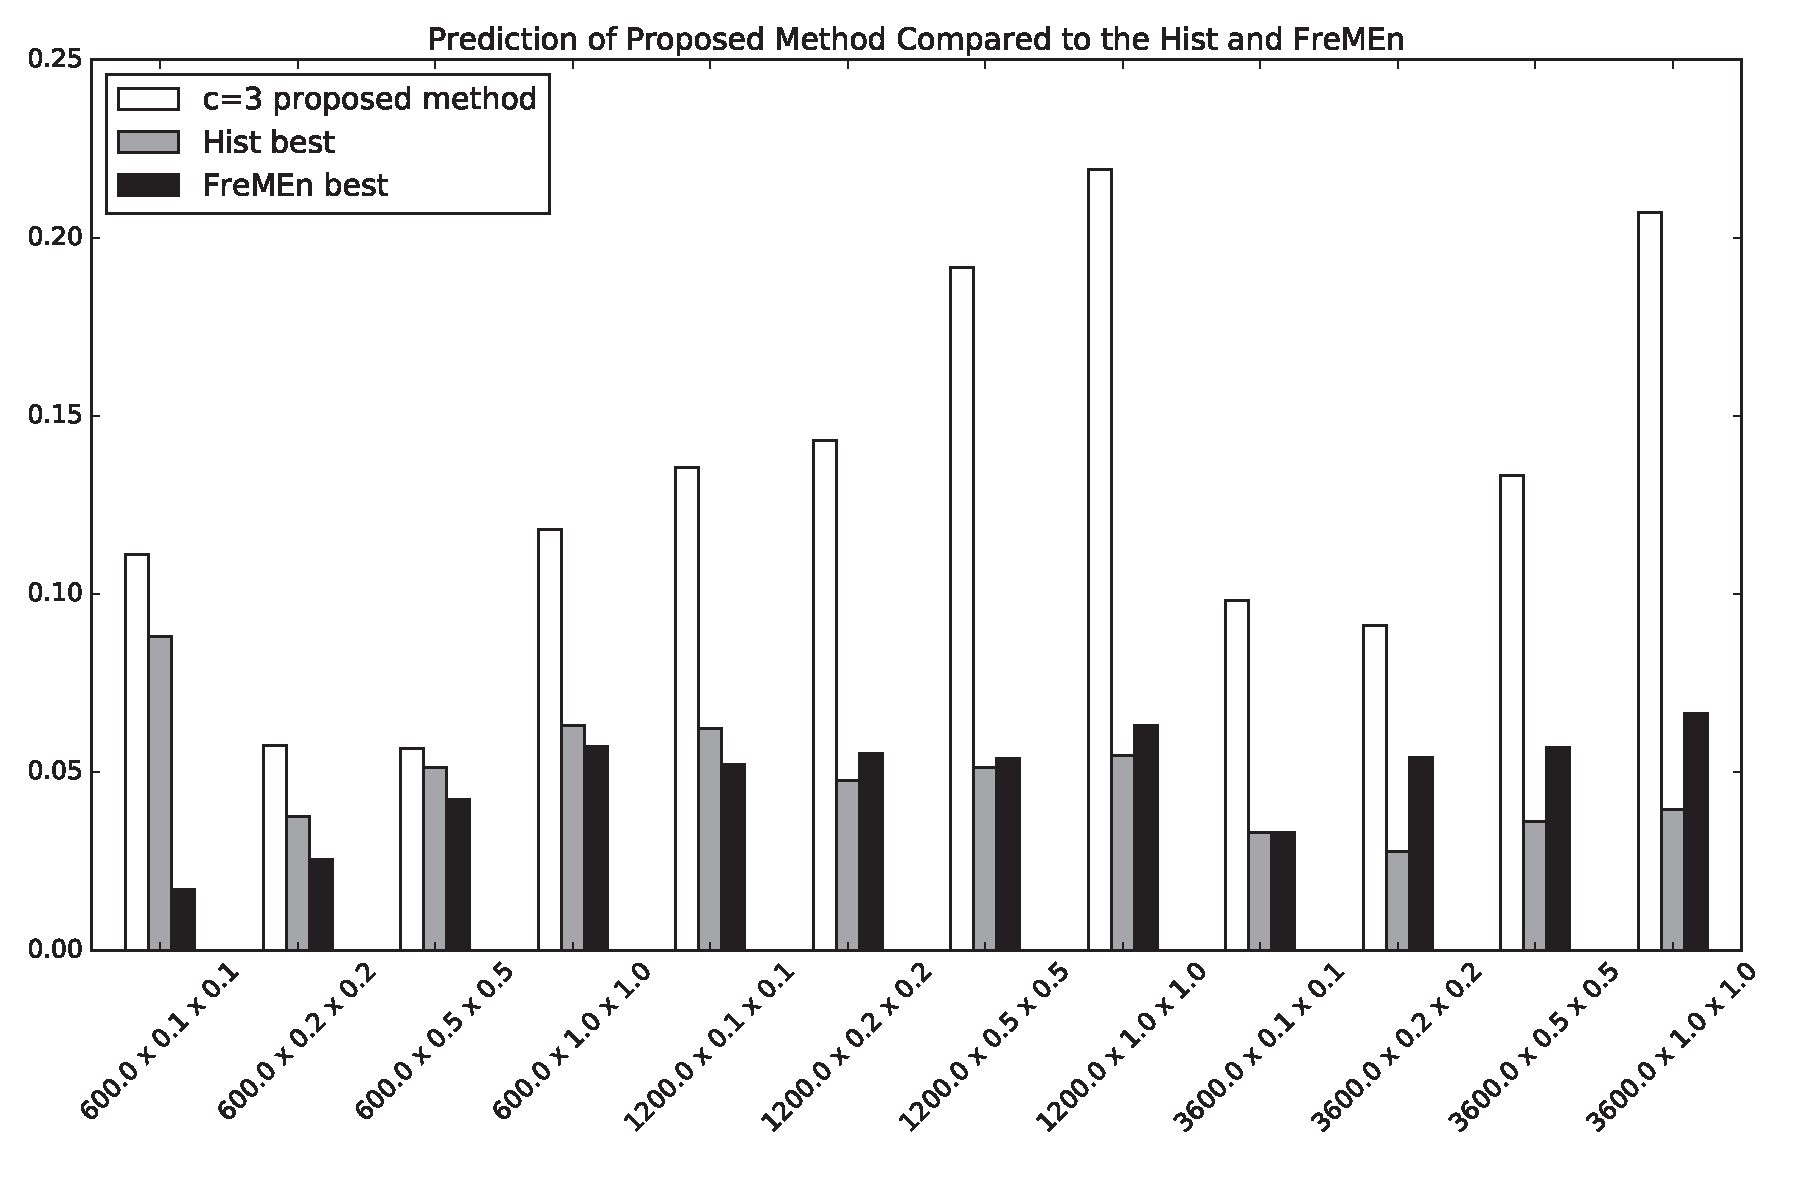
\includegraphics[width=0.7\columnwidth]{fig/ours3_hist_fremen.pdf}
    \caption{Comparison of predictive power of different methods. 
The graph shows the reduction of the prediction error compared to the \textit{Mean} model, which neglects the temporal properties of the people presence.
The indicated values ($y$-axes) are calculated using (\ref{eq:ratio}). 
On the $x$ axis, there are cell sizes or basic volumes.
White bar shows the prediction power of the proposed method using three clusters, grey bar Hist and black bar FreMEn.\label{graph:pedestrians}}
\end{center}
\end{figure}

It can be seen at Fig.~\ref{graph:pedestrians} that proposed method significantly outperforms the other ones. 
In most cases it is more than $5\%$ better than \textit{FreMEn} and \textit{Hist}.
%Fig~\ref{fig:model} also demonstrates that the predicted distributions of the people depend on time and follow the shape of the corridor (which is not part of the training data).
Moreover, the proposed model is much more memory efficient compared to FreMEn or the other models.
This is because our model is continuous and its complexity is not affected by the number of cells of the underlying grid, but it consists of positions of clusters $\left\{\mathbf{c}_{j}\right\},$ their weights $\left\{\alpha_{j}\right\},$ covariance matrices $\left\{\Sigma_{j}\right\},$ and a set of used periodicities $\left\{T_{\tau}\right\}$. 
For the two periods and three clusters it occupies $1.7$ KiB of memory space independently to the grid resolution.
In contrast to that, FreMEn needs several numbers for each modelled periodicity of every cell of the grid-based representation.
Thus, on our dataset, where the aforementioned grid has a resolution of $100,$ $50,$ $20,$ and $10$ cm, the FreMEn model occupies $1.1,$ $4.4,$ $27.2,$ and $108.9$ MiB of memory respectively, see Table \ref{tab:ram}.
In addition, the resolution of proposed method is derived from the cluster weights $\alpha_j.$ 
Therefore it is possible to store different resolutions of one model in almost no memory cost.

The downside of the proposed method is its computational complexity, which is caused primarily by the fact that the method is iterative.
While FreMEn calculates temporal model of all the grid cells in less than a minute, our method built the spatio-temporal model in an hour (CPU Intel Core i7-5005U).

\begin{table}[]
\caption{Memory Efficiency of Compared Methods}
\label{tab:ram}
\resizebox{0.7\textwidth}{!}{%
\begin{tabular}{ccccc}
\hline
\begin{tabular}[c]{@{}c@{}}resolution\\ {[}cm x cm{]}\end{tabular} & \begin{tabular}[c]{@{}c@{}}proposed method\\ c = 3, @ = 2\end{tabular} & \begin{tabular}[c]{@{}c@{}}FreMEn\\ f = 5\end{tabular} & \begin{tabular}[c]{@{}c@{}}Hist\\ h = 24\end{tabular} & Mean      \\ \hline
100 x 100                                                          & 1.7 KiB                                                                & 1.1 MiB                                                & 19.3 KiB                                              & 3.3 KiB   \\
50 x 50                                                            & 1.7 KiB                                                                & 4.4 MiB                                                & 307.3 KiB                                             & 12.9 KiB  \\
20 x 20                                                            & 1.7 KiB                                                                & 27.2 MiB                                               & 1.9 MiB                                               & 80.1 KiB  \\
10 x 10                                                            & 1.7 KiB                                                                & 108.9 MiB                                              & 7.7 MiB                                               & 320.1 KiB \\ \hline
\end{tabular}%
}
\end{table}





\subsubsection{Creation of Warped Hypertime Space in Detail}

At first, we partition the time line of the training set into $K$ discrete intervals $(t_{\kappa} ,t_{\kappa + 1})$.
Then, we predict a number of occurences within these time intervals by integrating values returned by our model over the entire domain of $\mathbf{x}$ and given time interval $(t_{\kappa} ,t_{\kappa + 1})$.
The obtained values form a histogram $\mathbf{m}$ representing the number of predicted occurences for each time interval $(t_{\kappa} ,t_{\kappa + 1})$.
Secondly, we count the number of training data $(\mathbf{x},t)$ occurring during $(t_{\kappa},t_{\kappa + 1})$, obtaining a histogram $\mathbf{h}.$
Then we calculate the differences of these histograms and create a new time series of residuals
%
\begin{equation}
R(t_k) = m_{\left(t_{\kappa} ,t_{\kappa + 1}\right)} - h_{\left(t_{\kappa} ,t_{\kappa + 1}\right)}.
\end{equation}
where $t_{k} \in \left(t_{\kappa}, t_{\kappa + 1}\right)$, $\kappa = 0, \ldots, K - 1.$
%
The frequency spectrum of the time series $R(t)$ is then processed by the non-uniform Fourier transform method \textit{FreMEn} described in~\cite{krajnik2017fremen}. 
Then we find the most prominent (i.e.\ with the largest absolute value) component $\gamma_{\tau}$ of the spectrum obtained from the previous step and calculate the corresponding period $T_{\tau}$ from its circular frequency $\omega_{\tau}$ as $T_{\tau} = 2\pi/\omega_{\tau}$. 

Once we have identified the dominant period $T_{\tau}$, we can extend the space with two extra dimensions.
For each $\left(\mathbf{x}_i, t_i\right)$ of the original measured data in space-time, we calculate its projection into the space extended by warped hypertime as follows:

\begin{equation}
\left(\mathbf{x}_i, t_i\right) \rightarrow \left(\mathbf{x}_i, \cos{\frac{2\pi t_{i}}{T_{\tau}}}, \sin{\frac{2\pi t_{i}}{T_{\tau}}}\right),
\end{equation}

where warped hypertime $\left(\cos{\frac{2\pi t_{i}}{T_{\tau}}}, \sin{\frac{2\pi t_{i}}{T_{\tau}}}\right)$ forms a circle in $2d$ plane which represent the periodicity and continuity of the occurences - the occurences with the similar position relative to periodicity $T_{\tau}$ are projected on the similar position on the circle.
%
%\begin{equation}\label{trans_cos}
%   {}^{cos}t_{i} = \cos{\frac{2\pi t_{i}}{T_{\tau}}},
%\end{equation}
%\begin{equation}\label{trans_sin}
%   {}^{sin}t_{i} = \sin{\frac{2\pi t_{i}}{T_{\tau}}}.
%\end{equation}
%
During the iterative process we can extend the extended vector space with another two dimensions and create a more dimensional warped hypertime extension of the space. 
Such projection of the measurements $\mathbf{x}_i$ obtained at time $t_i$ will be denoted ${}^{@}\mathbf{x}_{i},$ where:
%
\begin{equation}\label{eqn:extension}
    {}^{@+1}\mathbf{x}_{i} = \left({}^{@}\mathbf{x}_{i}, \,\cos{\frac{2\pi t_{i}}{T_{\tau_{@+1}}}}, \, \sin{\frac{2\pi t_{i}}{T_{\tau_{@+1}}}}\right),
\end{equation}
%
and ${}^{0}\mathbf{x}_{i} = \mathbf{x}_{i},$ ${}^{1}\mathbf{x}_{i} = \left(\mathbf{x}_{i}, \,\cos{\frac{2\pi t_{i}}{T_{\tau_1}}}, \, \sin{\frac{2\pi t_{i}}{T_{\tau_1}}}\right),$ ${}^{2}\mathbf{x}_{i} = \left(\mathbf{x}_{i}, \,\cos{\frac{2\pi t_{i}}{T_{\tau_1}}}, \, \sin{\frac{2\pi t_{i}}{T_{\tau_1}}}, \,\cos{\frac{2\pi t_{i}}{T_{\tau_2}}}, \, \sin{\frac{2\pi t_{i}}{T_{\tau_2}}}\right),$ etc.
%Corresponding set of projected measurements into the warped hypertime-space will be denoted as ${}^{@}\mathbf{X}.$ 
Fig~\ref{fig:hypertime}. taken from~\cite{removed} illustrates the warped hypertime projection of a number of human occurrences within a given area.
%
\begin{figure}
\begin{center}
    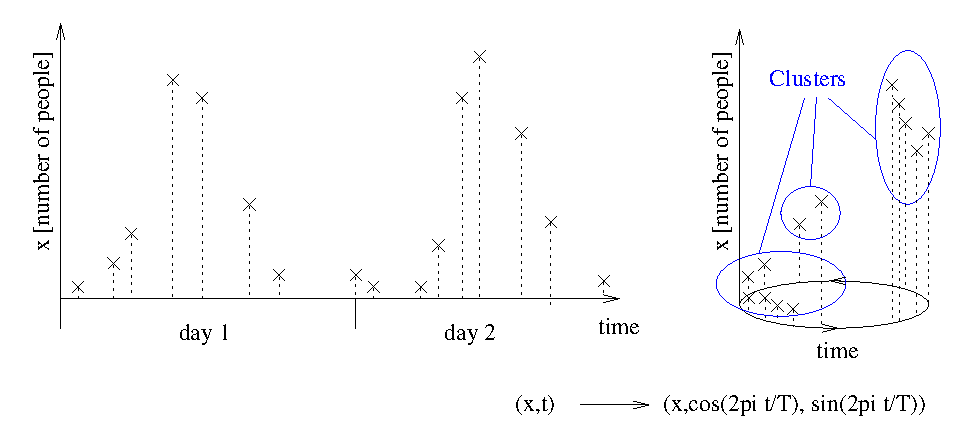
\includegraphics[width=0.7\columnwidth]{fig/hypertime1}
    \caption{Example of the warped hypertime projection. The measured tuples ($x_i,t_i$) are projected into a 3d vector space as ($x_i,cos(2\,\pi\,t_i/T),sin(2\,\pi\,t_i/T)$), where they form clusters because they exhibit a periodic behaviour with a period $T$. Obtained from~\cite{removed}.\label{fig:hypertime}}

\end{center}
\end{figure}


\subsection{Complex Control Experiments}

\begin{itemize}
    \item T.~Krajnik, T.~Vintr, S.~Molina, J.~P. Fentanes, G.~Cielniak, and T.~Duckett, ``Warped hypertime representations for long-term autonomy of mobile robots,'' \emph{arXiv preprint arXiv:1810.04285}, 2018.
    \item T.~Krajn{\'i}k, M.~Hanheide, T.~Vintr, K.~Kusumam, and T.~Duckett, ``Towards automated benchmarking of robotic experiments,'' in \emph{ICRA Workshop on  Reproducible Research in Robotics}, 2017.
\end{itemize}

In \cite{krajnik2018warped} we hypothesize that since the proposed model respects the spatio-temporal continuity of the modelled phenomena, it provides more accurate predictions than models that partition the modeled space into discrete elements. 
In this paper, we provide a description of the proposed method, and provide experimental evidence of its capability to efficiently represent spatio-temporal data and to predict future states of the environment.
Unlike the previous works~\cite{markov,rosen,kucner,fremen}, which can only introduce time into models that represent the environment by a discrete set of binary states, such as visibility of landmarks or cell occupancy in grids, our method is able to work with continuous and higher-dimensional variables, e.g.\ robot velocities, object positions, pedestrian flows, etc.
Moreover, the method explicitly represents and predicts not only the value of a given state, but also its probabilistic distribution at a particular time and location, which can be useful for task scheduling and planning~\cite{mudrova_ecmr15}.

Our experiments, based on real world data gathered over several weeks, confirm that the method achieved more accurate predictions than both static models and models that aim to represent time over a discretised space only.


???

The purpose of the experimental evaluation is to assess the predictive capability of the proposed method and its utility for different robotic tasks.
The performance of the method is evaluated in four different scenarios, which require predictions of variables of different dimensionalities.
The data for these experiments were collected by robotic sensors in real world conditions over periods of several weeks.
These scenarios correspond to our original motivational example from Section~\ref{sec:overview}, where we discussed how a long-term operating robot will benefit from the predictive capabilities of models that explicitly represent temporal behaviour of environment states with different dimensions.
To evaluate the efficiency of our method, we compare five different temporal models: \textit{Mean}, which predicts a value as an average of its past measurements, \textit{Hist\_n}, which divides each day into $n$ intervals and predicts the given variable as an average in a relevant time of a day, \textit{FreMEn\_m}, which extracts $m$ periodic components from the variable's history and uses these periodicities for prediction, \textit{HyT-EM\_k}, which uses the expectation-maximisation of $k$-component Gaussian Mixture Model over the hypertime space, and finally \textit{HyT-KN}, as described in Section~\ref{sec:discussion}.
The experimental evaluation is performed by an automated system~\cite{krajnik2017towards}, which first optimises each method's parameters (number of intervals $n$, number of periodicities $m$, and number of clusters $k$) and then runs a series of pairwise t-tests to determine which methods perform statistically significantly better than other ones.
To enable the reproducibility of the results, the evaluation system and the datasets are available online~\cite{fremen-www}.

\subsubsection{Door state}

The first scenario concerns a single binary variable, which corresponds to the state of a university office door.
The door was continuously observed by an RGB-D camera for 10 weeks to obtain the training set, and for another 10 weeks to obtain 10 testing sets, each one week long.
Since the RGB-D data processing was rather simple, the data contains noise, because people moving through the door caused the system to indicate incorrectly that the door was closed.

To compare the efficiency of the predictions, we calculated the mean squared error $\epsilon$ of the various temporal models' predictions $p(t)$ to the ground truth $s(t)$ as $\epsilon=\sqrt{\sum_T{(p(t)-s(t))^2}/|s(t)|}$.
%
\begin{figure}[!ht]
   \begin{center}
      \hfill
      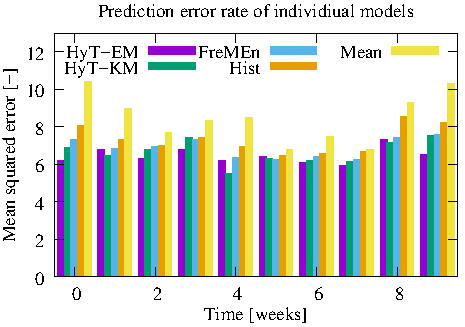
\includegraphics[height=3.0cm]{fig/door_graph}
      \hfill
      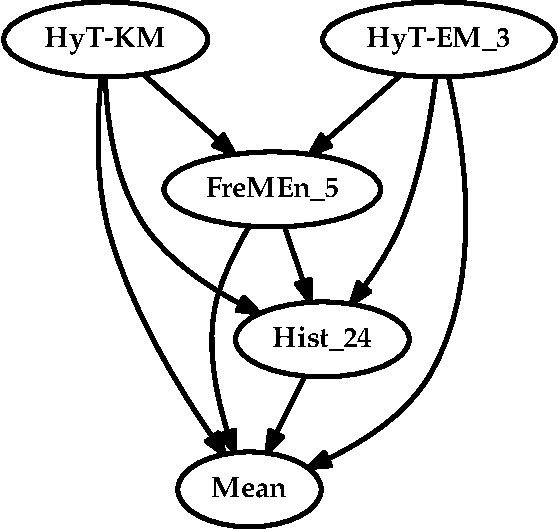
\includegraphics[height=3.0cm]{fig/door_stat}
      \hfill
      \caption{Door state prediction error. The left figure shows the MSE for the training (week 0) and testing (weeks 1-9) datasets. An arrow from model A to model B in the right figure indicates that A's prediction error is statistically significantly lower than prediction error of model B.\label{fig:binary}}
   \end{center}
\end{figure}
%
The results indicate that both hypertime-based models outperformed the other ones, including FreMEn~\cite{fremen}.
Both methods indicated that the most prominent periodicies corresponded to one day, four hours and one week. 

\subsubsection{Topological localisation}

In this scenario a robot has to determine its location in an open-plan university office based on the current image from its onboard camera and a set of pre-learned appearance models of several locations.
Since the appearance of these locations changes over time, it is beneficial to utilise appearance models that explicitly represent the appearance variations~\cite{prediction,fremen,rosen,churchill}.
This experiment compares the impact of different temporal models, which predict the visibility of environmental features at these locations, on the robustness of robot localisation. 
To gather data about the changes in feature visibility, a SCITOS-G5 robot visited eight different locations of the university office every 10 minutes for one week, collecting a training dataset with more than 8000 images.
After one week, the robot visited the same locations every 10 minutes for one day, collecting 1152 time-stamped images used for testing. 
% 
%\begin{figure}[!ht]
%   \begin{center}
%      \includegraphics[width=0.99\columnwidth]{fig/brayford.jpg}
%%%      \caption{Example images of the indoor training dataset. Shows the appearance of six monitored locations on November 2013.\label{pic:places}}
%   \end{center}
%\end{figure}
%
The training set images were then processed by the BRIEF method~\cite{brief}, which shows good robustness to appearance changes~\cite{krajnik2016griefras}. 
The extracted features belonging to the same locations were matched and we obtained their visibility over time, which was then processed by the temporal models evaluated.
Thus, we obtained a dynamic appearance-based model of each location that can predict which features are likely to be visible at a particular time.

During testing, the robot uses these models to calculate the likelihood of the features' visibility at each of the locations at the time it captured an image by its onboard camera (or extracted a time-stamped image from the testing set).
In particular, it selects the $n$ most likely-to-be-visible features at each location and time, matches these features to the features extracted from its onboard camera (or testing set) image, and determines the model with the most matches as its current location.
The localisation error is calculated as the ratio of cases when the robot incorrectly estimated its location to the total number of images in the testing set. 
The dependence of the average localisation error on the particular temporal model and number of features $n$ used for localisation is shown in Figure~\ref{fig:features}.
%
\begin{figure}[!ht]
   \begin{center}
   \hfill
      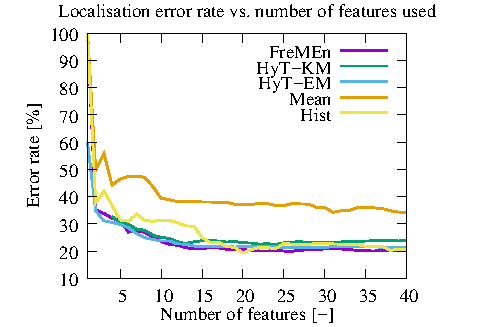
\includegraphics[height=3.0cm]{fig/localisation_graph}
      \hfill
      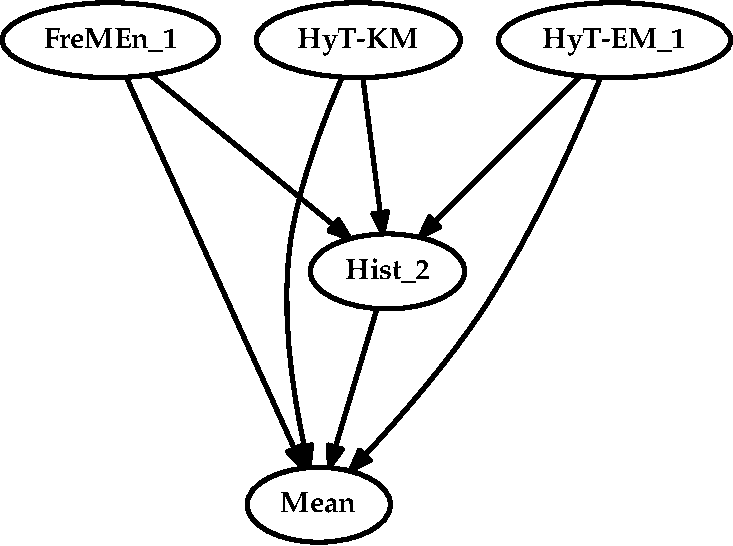
\includegraphics[height=2.95cm]{fig/localisation_stat}
      \hfill
      \caption{Temporal model performance for feature-based topological localisation. The left figure shows the dependence of localisation error rate on the number of features predicted by a given temporal model.
An arrow from A to B in the right indicates that A's localisation error rate is statistically significantly lower than localisation error rate of model B.\label{fig:features}}
   \end{center}
\end{figure}
%
The results indicate that the localisation robustness of the methods that take into account the rhythmic nature of the appearance changes outperform the \textit{Mean} method, which relies on the most stable image features.
Moreover, the methods that model these cyclic changes in a continuous manner perform better than the \textit{Hist} method which models different times of the day in separate, as shown in Figure~\ref{fig:features}. 

\subsubsection{Velocity prediction}

This scenario concerns the ability of our representation to predict the velocity of a robot while navigating through a given area, which depends on how cautiously it has to move due to the presence of humans.
Thus, this experiment is concerned with the ability of our method to predict a one-dimensional continuous variable (robot velocity) for a given time and location. 

The velocities and times of navigation for our evaluation were obtained from a database obtained with a SCITOS-G5 mobile platform, which gathered data in an open plan research office for more than 10 weeks.
Typically, the average velocity of the robot did not show much variation, but in cases it had to navigate close to workspaces and through doors, the velocity varied significantly.
To evaluate the ability of our approach to predict the robot velocity, we split the dataset into an 8-weeks long training set and two testing sets of 1-week duration.
%
\begin{figure}[!ht]
   \begin{center}
   \hfill
      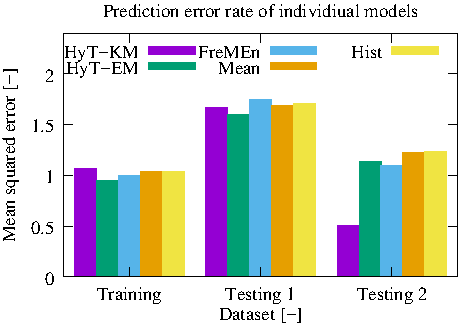
\includegraphics[height=2.9cm]{fig/nav_graph}
      \hfill
      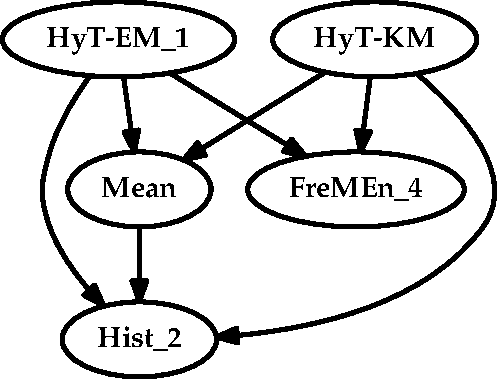
\includegraphics[height=2.5cm]{fig/nav_stat}
      \caption{Navigation velocity prediction error. The left figure shows the mean squared error for the training and testing sets.
An arrow from A to B in the right indicates that A's prediction error is statistically significantly lower than velocity prediction error of model B.\label{fig:navigation}}
   \end{center}
\end{figure}
%
As in the case of door state prediction, we calculated the mean square error of the predictions provided by our models, and compared them to find out which of the methods provide the most accurate predictions. 
Our results indicated that both Hypertime-based methods outperformed the other ones, as shown in Figure~\ref{fig:navigation}.

\subsubsection{Human presence}

Finally, we validated the proposed approach on 2-dimensional data indicating the positions of people in several corridors of the Isaac Newton Building at the University of Lincoln.
Data collection was performed by a mobile robot equipped with a Velodyne 3d laser rangefinder, which was placed at a T-shaped junction so that its laser range-finder was able to scan the three connecting corridors simultaneously.
To detect and localize people in the 3d point clouds provided by the scanner, we used an efficient and reliable person detection method~\cite{yan2017online}.
Since we needed to recharge the robot occasionally, we did not collect data on a 24/7 basis and recharged the robot batteries during nights, when the building is vacant and there are no people in the corridors.
Thus, our dataset spanned from early mornings to late evening over several weekdays.
Each day contains approximately $28000$ entries, which correspond to hundreds of walks by people through the monitored corridor. 
%
\begin{figure}[!ht]
   \begin{center}
   \hfill
      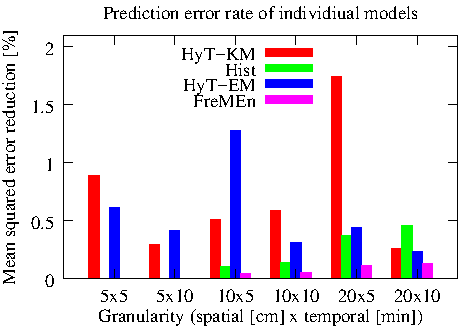
\includegraphics[height=3.0cm]{fig/ped_graph}
      \hfill
      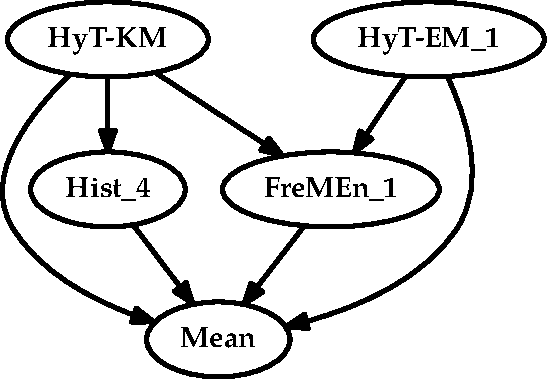
\includegraphics[height=2.8cm]{fig/ped_stat}
      \hfill
      \caption{Human presence prediction results. The left figure shows how the mean squared error reduced for a particular model compared to the \textit{Mean} model.
An arrow from A to B in the right indicates that A's prediction error is statistically significantly lower than velocity prediction error of model B.\label{fig:pedestrians}}
   \end{center}
\end{figure}
%
To quantitatively evaluate the model quality, we again split the gathered data into training and test sets, and learn the model from the training set only.
Then, we partition the timeline of the test data into a spatio-temporal 3d grid.
For each cell $g$, we count the number of detections $d_g$ that occurred and compare this value with the value $p_g$ predicted by a given spatio-temporal model.
To better visualise the methods' prediction improvements, we show the reduction of the mean square error compared to the $Mean$ model in Figure~\ref{fig:pedestrians}.
To make a comparison with other models, we apply the FreMEn method on each of the grid cells independently and then predict the most likely number of events at a given time in a particular cell.
Since the error is dependent on the partitioning used, we tested the method for grids of various cell sizes ranging from 5 to 20 cm and 5 to 30 minutes.

To demonstrate the model's ability to estimate the spatio-temporal distribution over time, we let it predict the most likely occurrence of people for different times.  
Figure~\ref{fig:spatemp} and video~\cite{video} show that the predicted distributions of the people depend on time and follow the shape of the corridor (which is not part of the training data). 

